\chapter{Triangulations}\label{cha:triangulations}
\ldots\todo[inline]{4 pages}

\todo[inline]{glue text}

\begin{definition}[Triangulation]
  Given the complete undirected graph
  \[ K_{|V|} = (V,E = \{e=\{v,w\} : v,w \in V \land v\not=w\}) \]
  of a vertex set \(V\) and a set of conflicts \(X \subseteq
  \{\{e_i, e_j\} : e_i,e_j \in E \land e_i \not= e_j\} \).
  A \emph{triangulation} \(T(V,X) \subseteq E\) of \(V\) with respect
  to \(X\) is a maximum set of non-conflicting edges:
  \[
    e_i \in T(V,X)
    \iff e_i \in E
    \land \forall e_j \in T(V,X) : \{e_i,e_j\} \not\in C
  \]
\end{definition}

\todo[inline]{glue text}

\begin{definition}[Conflict Graph]\label{def:conflict_graph}
  The conflict graph \(\gls{Gconf}[(E,X)] = (E,X)\) for a set of
  edges \(E\) and conflicts
  \(X \subseteq \{ \{e_i,e_j\} : e_i,e_j \in E \land e_i \not= e_j\}\)
  is an undirected graph with \(E\) as vertices and \(X\) as edges.
\end{definition}

\begin{figure}[ht]
  \centering
  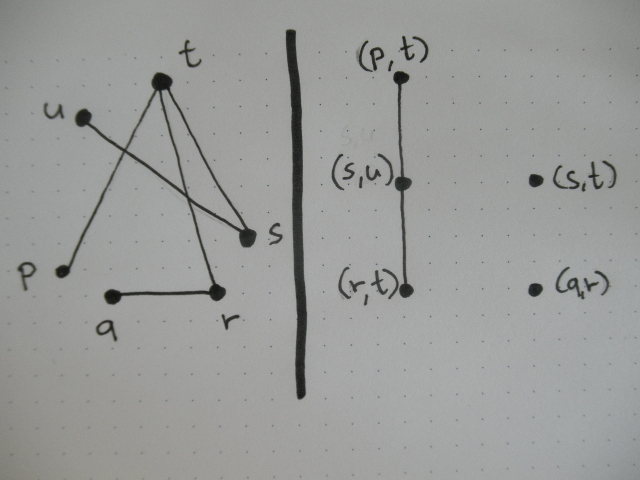
\includegraphics[width=0.5\textwidth]{img/example_conflict_graph.jpg}
  \todo[inline]{replace}
  \caption{Example of a conflict graph}
\end{figure}

\todo[inline]{glue text}

\begin{theorem}[Equality of Triangulation and Maximum Independent Set]
  \label{thm:triangulation_independent_set}
  Every triangulation \(T(V,X)\) of a vertex set \(V\) with respect
  to conflicts \(X\) is a maximum independent set for the conflict
  graph \(\gls{Gconf}[(E,X)]\) and vice versa. Hereby \(E\) are the
  edges of the complete undirected graph \(K_{|V|}\) for \(V\).
\end{theorem}

\begin{proof}
  \ldots\todo[inline]{proof}
\end{proof}

\begin{theorem}
  From
  \cref{thm:triangulation_independent_set}
  and
  \cref{thm:well_covered_minimum_independent_set}
  follows that finding the triangulation \(T(V,X)\) of a vertex set
  \(V\) with respect to conflicts \(X\) can be calculated in
  polynomial time.
\end{theorem}

\todo[inline]{glue text}

\begin{definition}[Triangulation with Forbidden Edges]
  A \emph{triangulation with forbidden edges} \(T(V,X,F)\) is a 
  triangulation of the vertex set \(V\) with respect to conflicts
  \(X\) which does not contain any of the edges in \(F\):
  \[ \forall e \in F : e \not\in T(V,X,F) \]
\end{definition}

\todo[inline]{glue text}

\begin{theorem}
  The decision problem whether a triangulation with forbidden edges
  \(T(V,X,F)\) exists is NP-complete.
  \todo[inline]{cite Lloyd: On Triangulations of a Set of Points in the Plane, triangulation existence problem}
\end{theorem}

\begin{definition}[Constrained Triangulation]
  \label{def:constrained_triangulation}
  \ldots\todo[inline]{definition}
\end{definition}

\section{Point Set Triangulations}

\todo[inline]{glue text}

\begin{definition}[Planar Points]
  A \emph{planar set of points} or \emph{set of points in the plane}
  \(P\) is a set of points with two coordinates:
  \[ P \subseteq \{p = (p_x,p_y) : p_x,p_y \in F\} \]
  We do not make any assumptions on the coordinates besides \(F\)
  being a field, e.g. the real numbers \gls{R}. Furthermore,
  because \(P\) is a set, no duplicate points \(p=(p_x,p_y)\in P\) and
  \(p'=(p_x',p_y')\in P\) with \(p_x=p_x'\) and \(p_y=p_y'\) are allowed.
  Note however that we do not require the points in \(P\) to be in 
  general position as that would forbid some interesting instances.
\end{definition}

\todo[inline]{glue text}

\begin{definition}[Line Segments]
  A \emph{line segment} \(s=(p,q)\) is determined by its endpoints
  \(p,q\in P\) with \(P\) being a point set. For compatibility
  with other definitions, \(s\) is directed from \(p\) to \(q\), i.e.
  \((p,q)\not=(q,p)\) and contains all points ``between'' \(p\) and
  \(q\):
  \[ m \in s \iff \exists a\in [0,1] : m = p + a \cdot (q-p) \]
\end{definition}

\todo[inline]{glue text}

\begin{definition}[Crossing]\label{def:crossing}
  Two line segments \(s_i=(p_i,q_i)\) and \(s_j=(p_j,q_j)\) with 
  different slope are \gls{cross}, if their intersection is not empty
  and not an endpoint, i.e.
  \[
    s_i, s_j~\gls{cross}
    \iff
    (p = s_i\cap s_j) \land
    (|s_i\cap s_j| = 1) \land
    (p \not\in \{p_i,q_i,p_j,q_j\})
  \]

  Two segments \(s_i\) and \(s_j\) are \gls{ncross} if they are
  not \gls{cross}. A set \(S\) of segments is \gls{cross} if at least
  two segments \(s_i, s_j \in S\) are \gls{cross}. It is \gls{ncross}
  if each pair \(s_i, s_j \in S\) is \gls{ncross}.
\end{definition}

\todo[inline]{glue text}

\begin{definition}[Overlapping Segments]
  \label{def:overlapping_segments}
  Given a point set \(P\) and a line segment \(s = (p,q)\) with
  \(p,q \in P\). \(s\) is \gls{overlap} in \(P\) iff there is a point
  \(p' \in P\) which lies in its interior:
  \[
    s~\gls{overlap}
    \iff  \exists p' \in P : (p' \in s) \land (p' \not\in \{p,q\})
  \]
  \(s\) is \gls{noverlap} if it is not \gls{overlap}.
\end{definition}

\begin{figure}[ht]
  \centering
  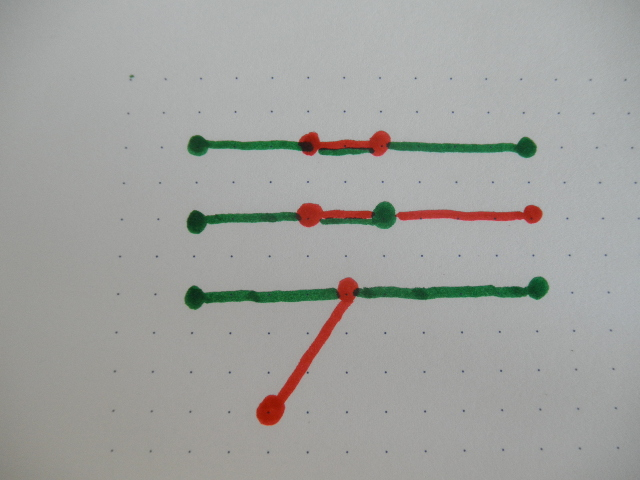
\includegraphics[width=0.5\textwidth]{img/example_overlapping.jpg}
  \todo[inline]{replace}
  \caption{Examples of overlapping segments.}
\end{figure}

\todo[inline]{glue text}

\begin{definition}[Topological Representation]
  A vertex set \(V(P)\) represents a point set \(P\) iff there
  is exactly one vertex \(v_p \in V(P)\) for each point \(p \in P\)
  and \(v_p\) can be identified by \(p\) and vice versa.
%   
%   An edge set \(E(S)\) represents a set of line segments \(S\) iff
%   there is exactly one edge \(e_s = \{v_p, v_q\} \in E(S)\) for each 
%   line segment \(s = (p,q) \in S\) and \(e_s\) can be identified by
%   \(s\) and vice versa. The endpoints \(p\) and \(q\) of \(s\) are 
%   represented by the vertices \(v_p\) and \(v_q\), respectively. We
%   hereby assume that not \((p,q) \in S\) and \((q,p) \in S\) as they
%   would be represented by the same edge.
\end{definition}

\begin{definition}[Point Set Triangulation]
  \label{def:point_set_triangulation}
  The triangulation \(T(P)\) of a point set \(P\) is a triangulation
  with forbidden edges \(T(P) = T(V,X,F)\) where the vertex set
  \(V=V(P)\) represents \(P\), the conflicts \(X\) are all
  \gls{cross} segments and the forbidden edges \(F\) are the
  \gls{overlap} segments:
  \begin{alignat*}{1}
    \left\{ \{v_p,v_q\}, \{v_{p'},v_{q'}\} \right\} \in X
    &\iff (p,q), (p',q')~\gls{cross} \\
    \{v_p,v_q\} \in F
    &\iff (p,q)~\gls{overlap}
  \end{alignat*}

  For convenience we define \(s=(p,q) \equiv e=\{v_p,v_q\}\) such
  that \(s \in T(P) \iff e \in T(P)\). For a slightly different yet
  equivalent definition of a point set triangulation see also
  \cite[Section 9.1]{deberg_compgeom}. Note that for \(P\) in general
  position \(F\) is empty.
\end{definition}

\begin{theorem}
  A point set triangulation can be calculated in polynomial time.
\end{theorem}

\begin{proof}
  \ldots\todo[inline]{proof}
\end{proof}

\begin{definition}[Constrained Point Set Triangulation]
  \label{def:constrained_point_set_triangulation}
  \ldots\todo[inline]{definition}
\end{definition}

\begin{theorem}
  A constrained point set triangulation can be calculated in polynomial time.
\end{theorem}

\begin{proof}
  \ldots\todo[inline]{proof}
\end{proof}

%---------------------------------------------------------------------##########

% One day Greg had art class and the children were given sheets of
% paper with points on them. The task was to connect all the points 
% such that they have as many bounded areas as possible. Greg 
% connected all the points taking care that the connections would only 
% intersect in the given points. He was happy to see that the result 
% consisted only of triangles filling up the whole space within the 
% points. Also he had more bounded areas than any other child --- 
% even more than Joey who filled up his sheet with quadrangles. Greg's
% teacher, Mrs. Minerva, told him that he made a triangulation.
% 
% After seeing Greg's sheet, some of his friends let their connections
% cross each other to get more areas, but Greg considered that
% cheating. To stay the winner of the competition he made a new rule
% that no point connections are allowed to cross.
% 
% Joey tried to circumvent Greg's rule by adding new points to his
% sheet. For each new point he added on the outside he could make
% several new connections and therefore got soon many more areas. So
% Greg had to quickly come up with another rule only allowing the
% existing points to take part of the competition.
% 
% \begin{definition}[Induced Segments]\label{def:induced_segments}
%   The set of induced line segments \(S_P\) of a planar point set \(P\)
%   consists of all \gls{noverlap} unique line segments having
%   endpoints in \(P\):
%   \[
%     S_P := \{s=(p,q) \in P^2 : (p < q) \land s~\gls{noverlap}\}
%   \]
%   Let \(<\) hereby denote the lexicographical order, that is for
%   \(p = (p_x,p_y)\) and \(q = (q_x,q_y)\):
%   \[
%     p < q \iff (p_x < q_x) \lor ((p_x = q_x) \land (p_y < q_y)).
%   \]
% \end{definition}
% 
% With those two new rules no one could think of a better way to make
% areas than Greg's triangles. Even Mrs. Minerva said that under those
% conditions it would not be possible to come up with a subdivision
% which has more faces than a triangulation.
% 
% \begin{verbatim}
%   - observation: when changing geometry but not topology,
%     certain properties stay the same
%   - e.g. angle/area/length preserving transformation
%     => many optimal triangulations map to one topological
%     (size doesn't matter)
% \end{verbatim}
% \todo[inline]{notes}

\section{Polygon Triangulations}
\todo[inline]{definitions (and related work?)}

\section{Edge Flipping}
\begin{verbatim}
  - what is a flip?
  - flip graph complexity
  - local vs. global optimal
  - hint to edge flipping paper
\end{verbatim}
\todo[inline]{notes}

\section{Related Work}
After class was over, Greg asked Mrs. Minerva if there are different
kinds of triangulations. She replied that the problem of 
triangulating has kept researchers busy for over 100 years already
\cite{triangulation_hilbert} and that people have found different
aspects in that a triangulation can be optimal.

The most famous class is the Delaunay triangulation
\cite[Section 9.2]{deberg_compgeom}. It forces every circumcircle
of a triangle to be empty of other points and therefore maximizes
the minimum angle \cite[Theorem 9.9]{deberg_compgeom}. There is an
edge flipping algorithm which calculates it in \(O(n \log n)\) 
expected time using \(O(n)\) space 
\cite[Theorem 9.12]{deberg_compgeom}.

There are several other triangulations which can be computed in
polynomial time. Minimizing the maximum edge length in \(O(n^2)\)
times was one of the first results \cite{triangulation_minmax_length}.
The counterpart of a Delaunay triangulation, 
minimizing the maximum angle, takes \(O(n^2 \log n)\) time and
\(O(n)\) space \cite{triangulation_edge_insertion}. The same
approach can also produce triangulations which maximize the minimum 
height of a triangle. Finally, the same reference shows also that 
minimizing the maximum slope and minimizing the maximum eccentricity 
can both be done in \(O(n^3)\) time and \(O(n^2)\) space. A 
triangulation which minimizes or maximizes the area of triangles can
be computed in \(O(n^2 \log n)\) time with \(O(n^2)\) space.
\cite{triangulation_area}

Other triangulations have been proven NP-hard or NP-complete. One
of them is to minimize the edge length sum (also known as the minimum
weight triangulation) which is NP-hard \cite{mwt_complexity}. 
Maximizing the minimum edge length was stated an open problem
\cite{triangulation_minmax_length} but 20 years later it has been
shown that it is NP-complete \cite{mmlt_complexity}. The latter one
remains NP-hard for polygons with holes and interior points
\cite{mmlt_polygons} but can be solved in \(O(n^3)\) time for simple
polygons and even in linear time for convex polygons
\cite{mmlt_convex_polygons}.

%---------------------------------------------------------------------##########
